\chapter{Testes de Verificação e Validação}
\label{testes}

\section{Características Gerais}

Este capítulo apresenta os testes de verificação e validação realizados no projeto Micromouse, com o objetivo de avaliar se os subsistemas desenvolvidos atendem aos requisitos definidos e se, quando integrados, são capazes de operar de forma coerente com a proposta do produto. Os ensaios contemplam aspectos estruturais, eletrônicos, energéticos, de software e de integração global, considerando tanto a análise individual dos componentes quanto o comportamento do sistema completo.

\section{Testes da Estrutura}

Esta seção apresenta os ensaios e metodologias de verificação e validação aplicados ao ecossistema estrutural do Micromouse. O propósito fundamental desta etapa consiste em assegurar que o chassi manufaturado e o ambiente de testes físico repliquem com fidelidade as premissas analíticas estabelecidas no projeto conceitual. Para tanto, avaliam-se parâmetros críticos de tolerância dimensional, estabilidade cinemática, rigidez a impactos e a dinâmica de rolamento do sistema de locomoção.

\subsection{Inventário Físico e Conformidade de Peças}

O primeiro estágio de verificação consistiu na conferência e inspeção individual dos componentes estruturais manufaturados antes da integração final do sistema. A Figura~\ref{fig:pecas_separadas} apresenta o inventário físico dos elementos mecânicos brutos obtidos por impressão 3D em PLA, dispostos em bancada para fins de verificação de qualidade.

A análise visual das peças físicas revela um alto nível de fidelidade geométrica na deposição das camadas de filamento, mantendo a integridade estrutural das furações concêntricas de fixação dos motores e dos encaixes dos rolamentos das rodas. Na imagem, observa-se o conjunto básico de sustentação e transmissão do robô, composto pelas duas seções principais do chassi (base inferior de fixação e estrutura superior de proteção), 4 unidades de rodas com sulcos para acoplamento de pneus e 2 engrenagens cilíndricas de dentes retos destinadas à redução e transmissão do sistema motriz.

\begin{figure}[htbp]
    \centering
    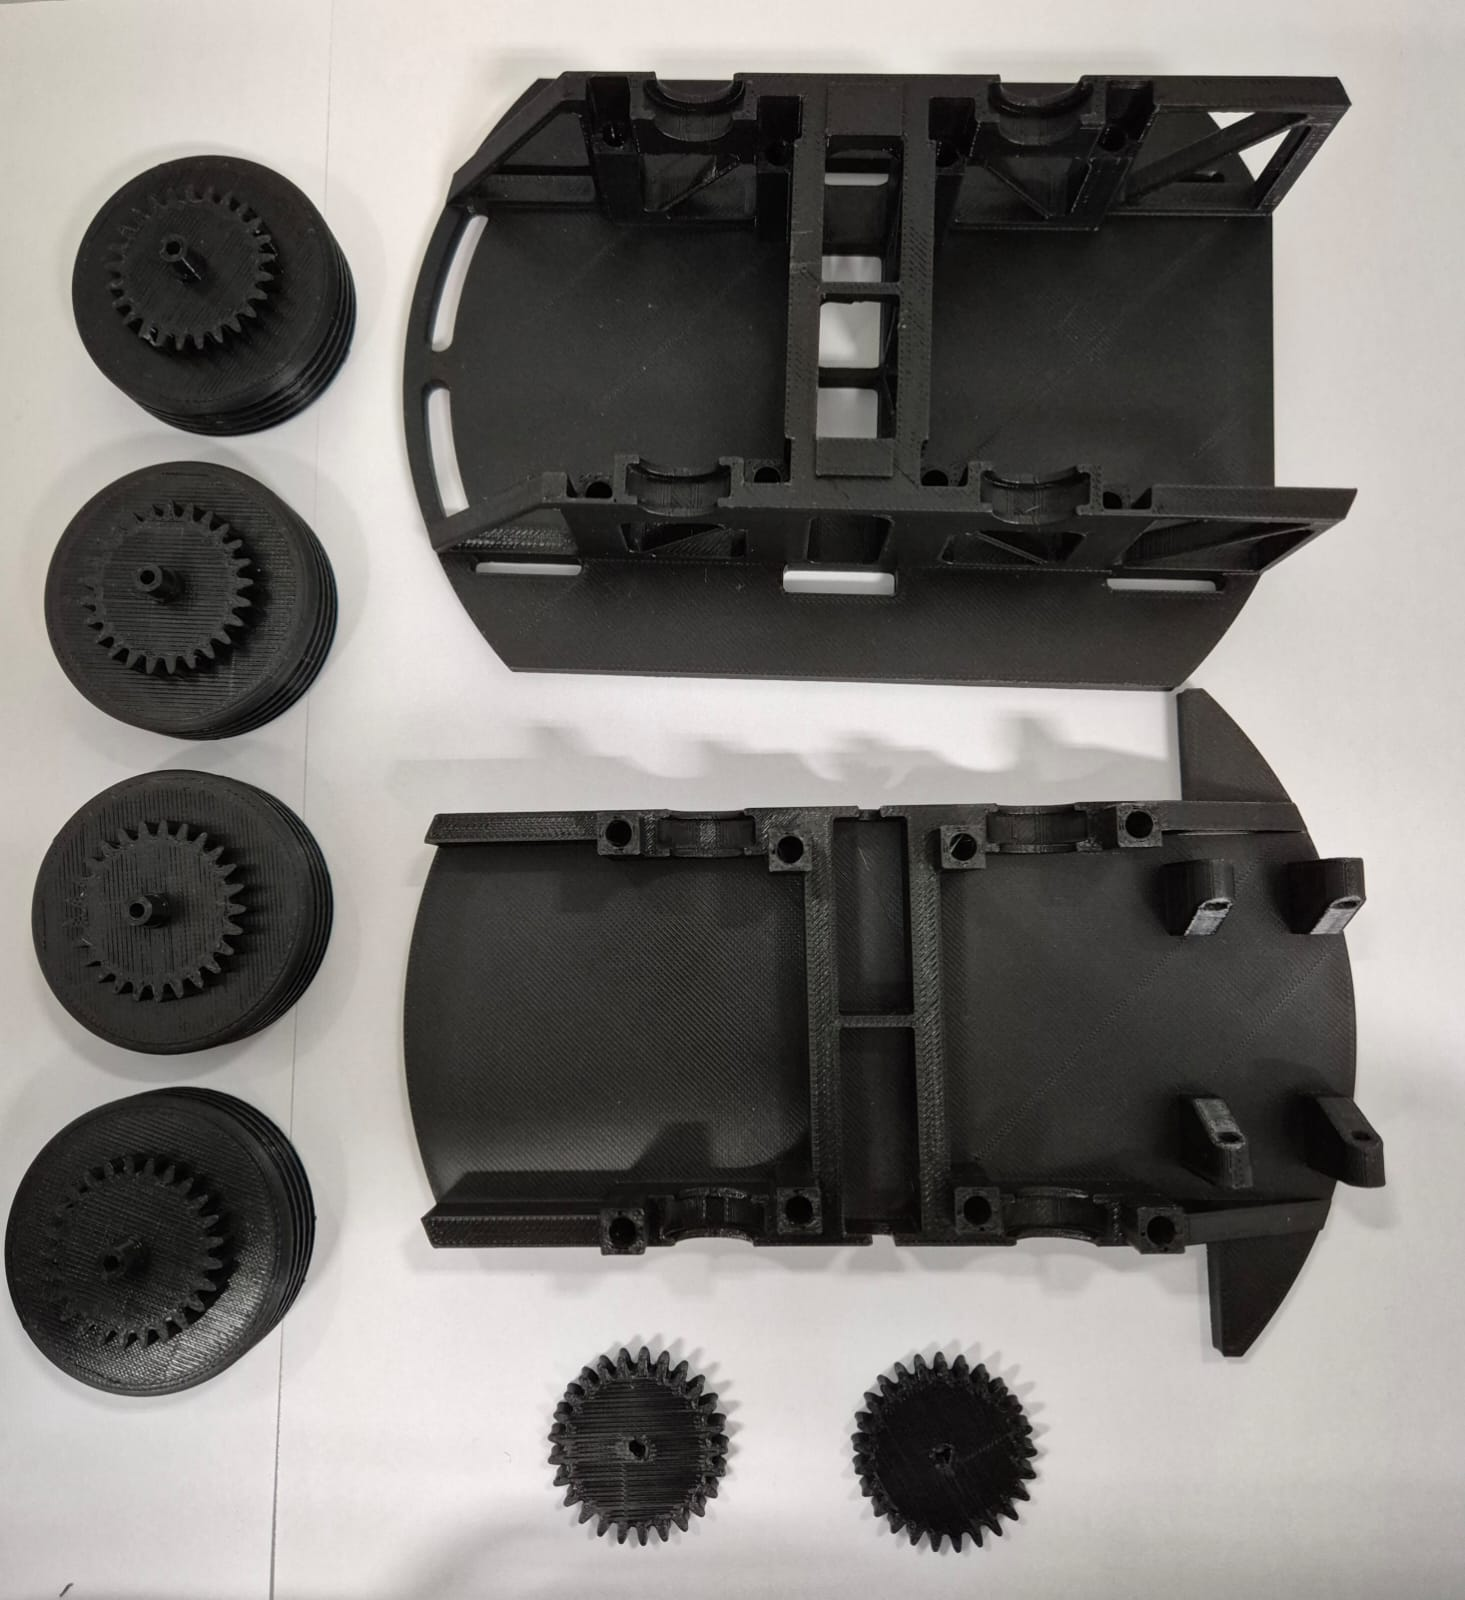
\includegraphics[width=0.55\textwidth]{figuras/pecas_separadas.jpeg}
    \caption{Componentes estruturais e mecânicos do micromouse manufaturados em PLA.}
    \label{fig:pecas_separadas}
\end{figure}

Para fins de rastreabilidade e controle de qualidade industrial, a disposição e a correta identificação geométrica de cada um desses 8 subsistemas podem ser correlacionadas diretamente com o diagrama técnico de detalhamento e a listagem estruturada presentes na Figura~\ref{fig:Draft Micromouse explodido}.

\subsubsection{Montagem Estrutural e Consistência com o Modelo CAD}

Após o inventário inicial, executou-se a montagem mecânica do chassi para análise de rigidez e acoplamento. A Figura~\ref{fig:estrutura_montada} ilustra a carcaça do Micromouse montada, evidenciando o posicionamento preliminar de componentes de fiação e elementos eletrônicos internos em seus respectivos nichos de fixação. Para assegurar a estabilidade mecânica do conjunto e mitigar vibrações estruturais que possam comprometer as leituras dos sensores, a união entre os planos estratificados foi realizada de forma híbrida, empregando guias de encaixe por pressão integradas ao design do PLA em conjunto com elementos de fixação roscados (parafusos metálicos passantes).

\begin{figure}[htbp]
    \centering
    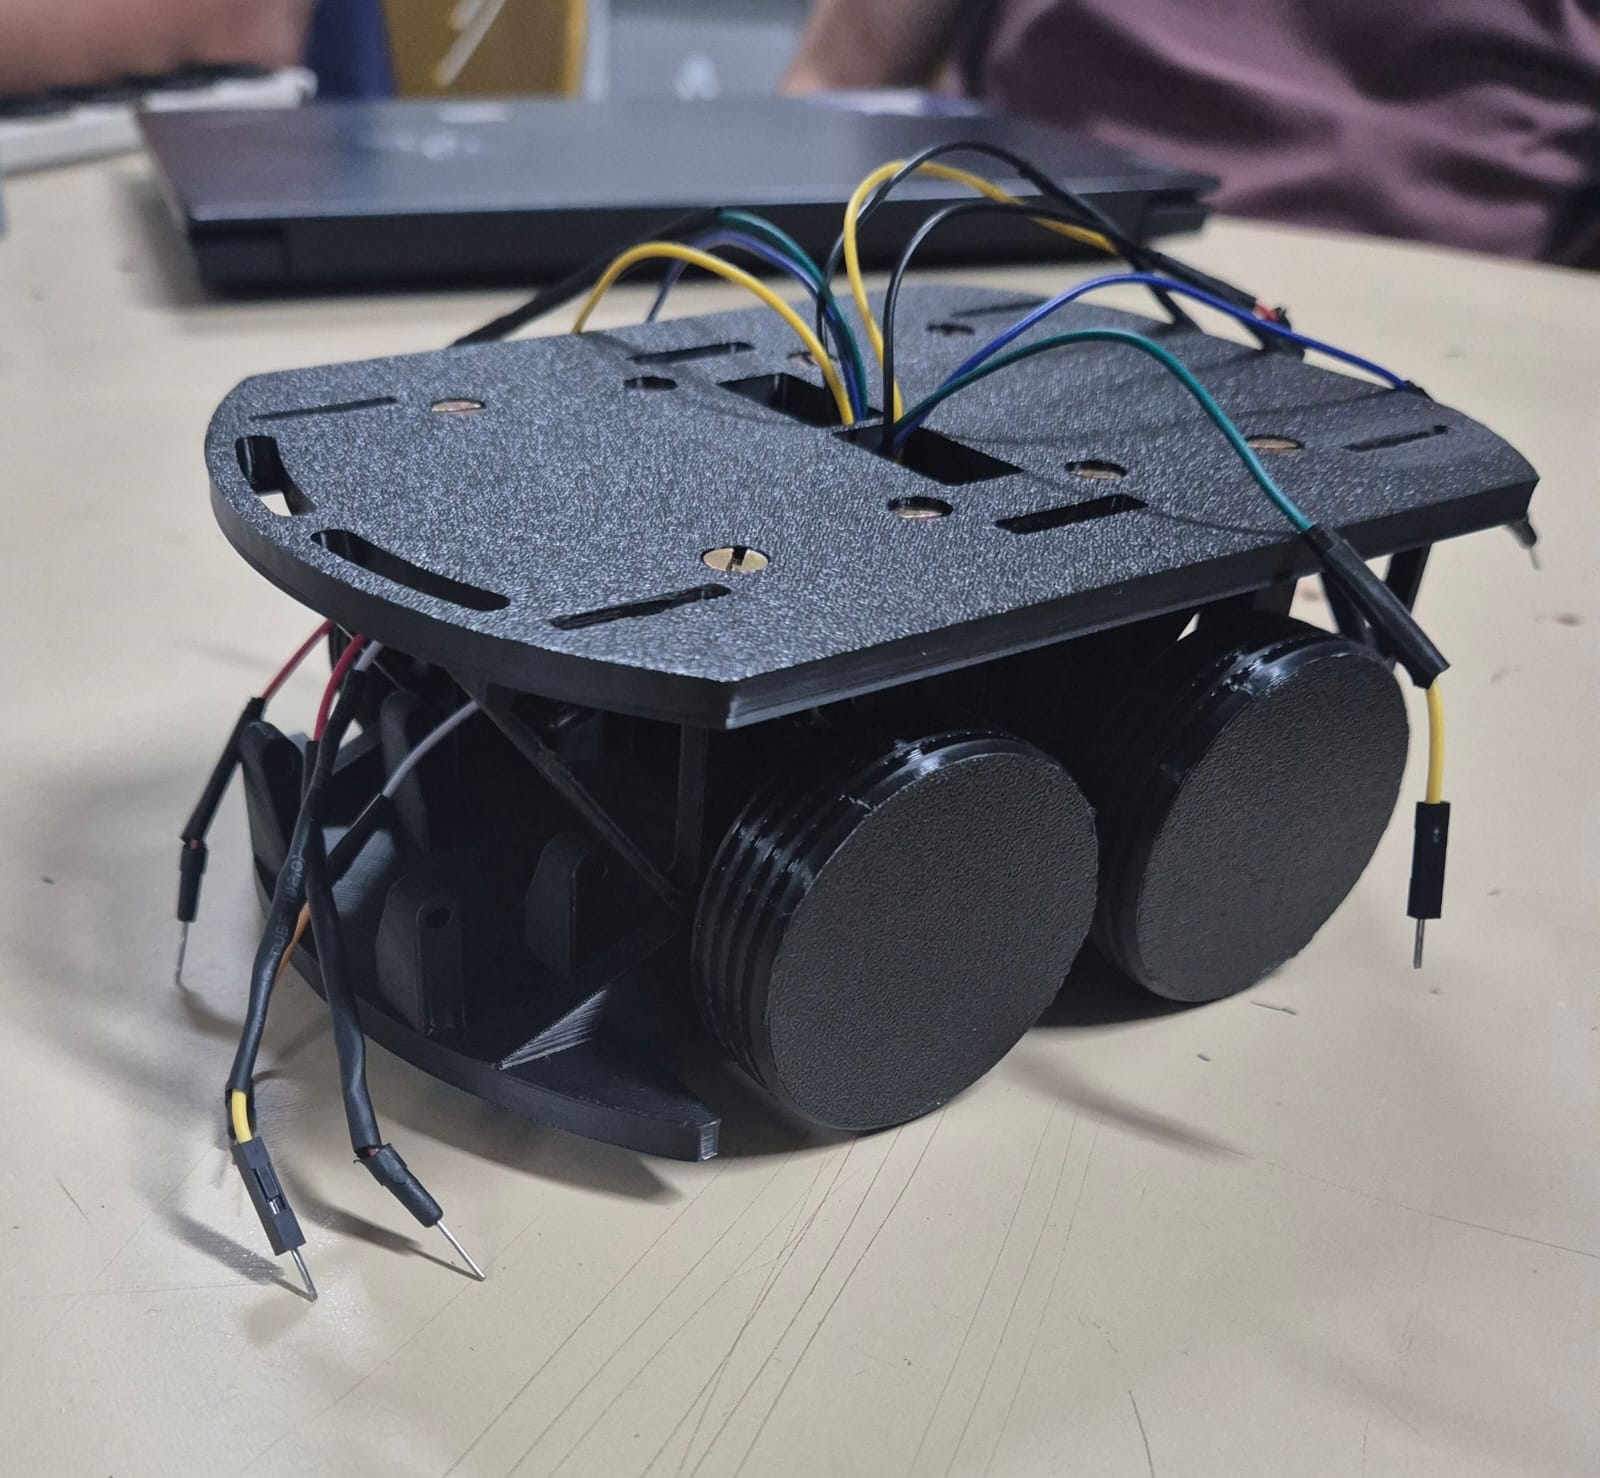
\includegraphics[width=0.55\textwidth]{editaveis/estrutura_montada.jpeg}
    \caption{Estrutura do chassi montada com parafusos e encaixes, com fiação e hardware interno preliminar.}
    \label{fig:estrutura_montada}
\end{figure}

Essa configuração física comprova a eficiência do projeto estrutural em prover proteção passiva aos componentes internos, mantendo o acesso para manutenção prático. Para certificar que a execução real não divergiu das premissas geométricas teóricas, o protótipo montado foi confrontado com o ambiente virtual. A Figura~\ref{fig:carro_cad} expõe o modelo tridimensional renderizado em ambiente CAD, servindo como ferramenta de controle de qualidade para atestar que as furações concêntricas de união, os suportes de sensoriamento e as folgas de acoplamento foram rigorosamente respeitados. A validação dessa montagem estratificada toma como referência técnica a vista explodida oficial do projeto, documentada detalhadamente no desenho técnico presente na Figura~\ref{fig:Draft Micromouse explodido}.

\begin{figure}[htbp]
    \centering
    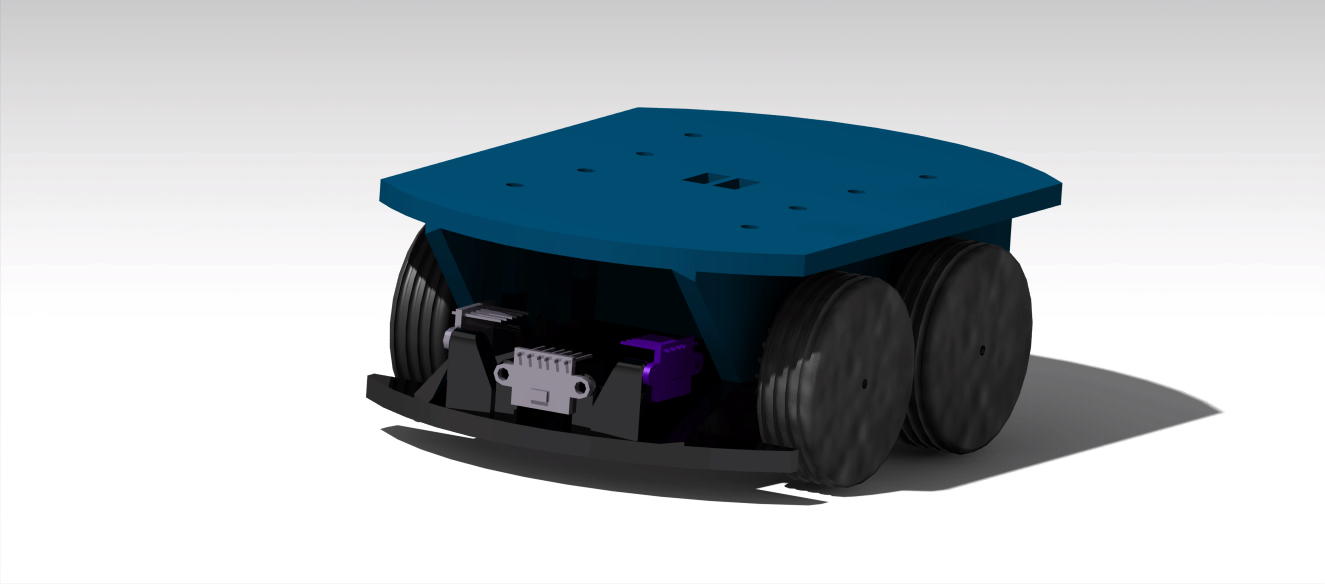
\includegraphics[width=0.75\textwidth]{editaveis/carro_cad.jpg}
    \caption{Ilustração do veículo completamente montado em ambiente virtual CAD.}
    \label{fig:carro_cad}
\end{figure}

\subsection{Ensaios de Verificação Dimensional e de Tolerâncias}
Utilizando instrumentos de medição de precisão (paquímetro), aferiu-se o envelope volumétrico final do robô montado. Os resultados confirmaram que o chassi manteve a largura nominal de $110 mm$ e o comprimento de $156 mm$ dentro de uma margem de tolerância física de $\pm 0,5mm$, validando a conformidade com o projeto conceitual e o CAD elaborado.

Estas dimensões críticas e os limites de tolerância adotados na fabricação foram validados e estão devidamente cotados nas projeções ortogonais (vistas superior, lateral e seções transversais) localizadas na Figura~\ref{fig:carro_cad}.

\subsection{Validação de Locomoção, Rodas e Rolamentos}
O sistema de suspensão estática e acoplamento dos eixos passou por ensaios cinemáticos para verificar o alinhamento das rodas e a eficiência dos rolamentos. O conjunto apresentou baixo coeficiente de fricção interna, assegurando que o torque fornecido pelos motores GA12-N20-S0310D-E seja eficientemente convertido em força trativa.

\subsection{Testes Dinâmicos de Curvas no Labirinto}

O robô foi submetido a ensaios práticos de rotação de $90^{\circ}$ e deslocamentos em trajetórias diagonais dentro do labirinto modular. Inicialmente, o teste comprovou empiricamente o cálculo teórico de folga espacial lateral, estabelecido em $\le 16,80 cm$. O arranjo recuado do sistema de rodagem e o chanfro projetado nas extremidades do chassi mostraram-se eficazes em evitar colisões ou raspagens contra as paredes do ambiente de testes durante manobras controladas em baixa velocidade.

Contudo, observou-se que o comprimento diagonal total do Micromouse é de $160 mm$, o que estabelece uma margem geométrica extremamente estreita e intolerante a pequenas derivas ou erros de alinhamento cinemático. Diante do risco iminente de colisões durante transições rápidas, os ensaios dinâmicos atuaram como um balizador para decisões de projeto. 

Como ação corretiva e de otimização para o próximo ponto de controle, determinou-se a reestruturação e o rearranjo dos componentes eletrônicos dispostos interna e externamente na estrutura estratificada. Essa reorganização do leiaute visa otimizar o espaço interno dedicado ao acondicionamento dos módulos, viabilizando a diminuição do raio dimensional do chassi e, por consequência, contraindo a sua diagonal geométrica. Como resultado, o Micromouse obterá uma margem de segurança significativamente maior contra colisões, garantindo a estabilidade operacional e a integridade do robô durante curvas e manobras severas em alta velocidade. Ressalta-se que tais modificações estruturais serão conduzidas de modo a respeitar estritamente a identidade visual, a distribuição de massas e as diretrizes funcionais consolidadas no projeto conceitual.

\subsection{Ensaio de Resistência a Impactos}
Por fim, realizou-se um teste de resistência passiva estrutural submetendo o chassi a pequenas colisões frontais e laterais simuladas em velocidade nominal. A estrutura absorveu satisfatoriamente a energia cinética dos impactos devido à flexibilidade controlada e preenchimento interno do filamento PLA, garantindo proteção total aos sensores ToF e circuitos internos sem apresentar trincas, fraturas ou folgas nos encaixes da tampa superior.

\section{Testes de \textit{hardware}}

Essa seção tem como principal objetivo explicitar os testes de \textit{hardware} realizados para a construção e funcionamento do MicroMouse. Dessa forma, apresentaremos os testes de processamento, sensores, armazenamento e comunicações.

\subsection{Processamento - ESP32}

A interface de desenvolvimento escolhida pela equipe foi a \textbf{ESP-IDF}. A escolha se deu, principalmente, por afinidade de alguns membros do grupo de eletrônica. Além disso, a interface possui amplo suporte a todas as funcionalidades da ESP32 que serão utilizadas, e boa integração com o Visual Studio Code, o editor de código utilizado pela equipe. 

Assim, foi rodado um exemplo mínimo no qual testamos a ESP32 para fazer a rotação simples de um dos motores, na primeira montagem realizada pela equipe. O teste resultou em sucesso e conseguiu-se acionar o motor via ESP32. Esse teste pode ser encontrado na Figura \ref{fig:exemploMin}.

Após isso, também fizemos os testes com os dois atuadores, os motores, realizando testes de mudança de direção e velocidade, sendo todos bem sucedidos.

\begin{figure}[htbp]
    \centering
    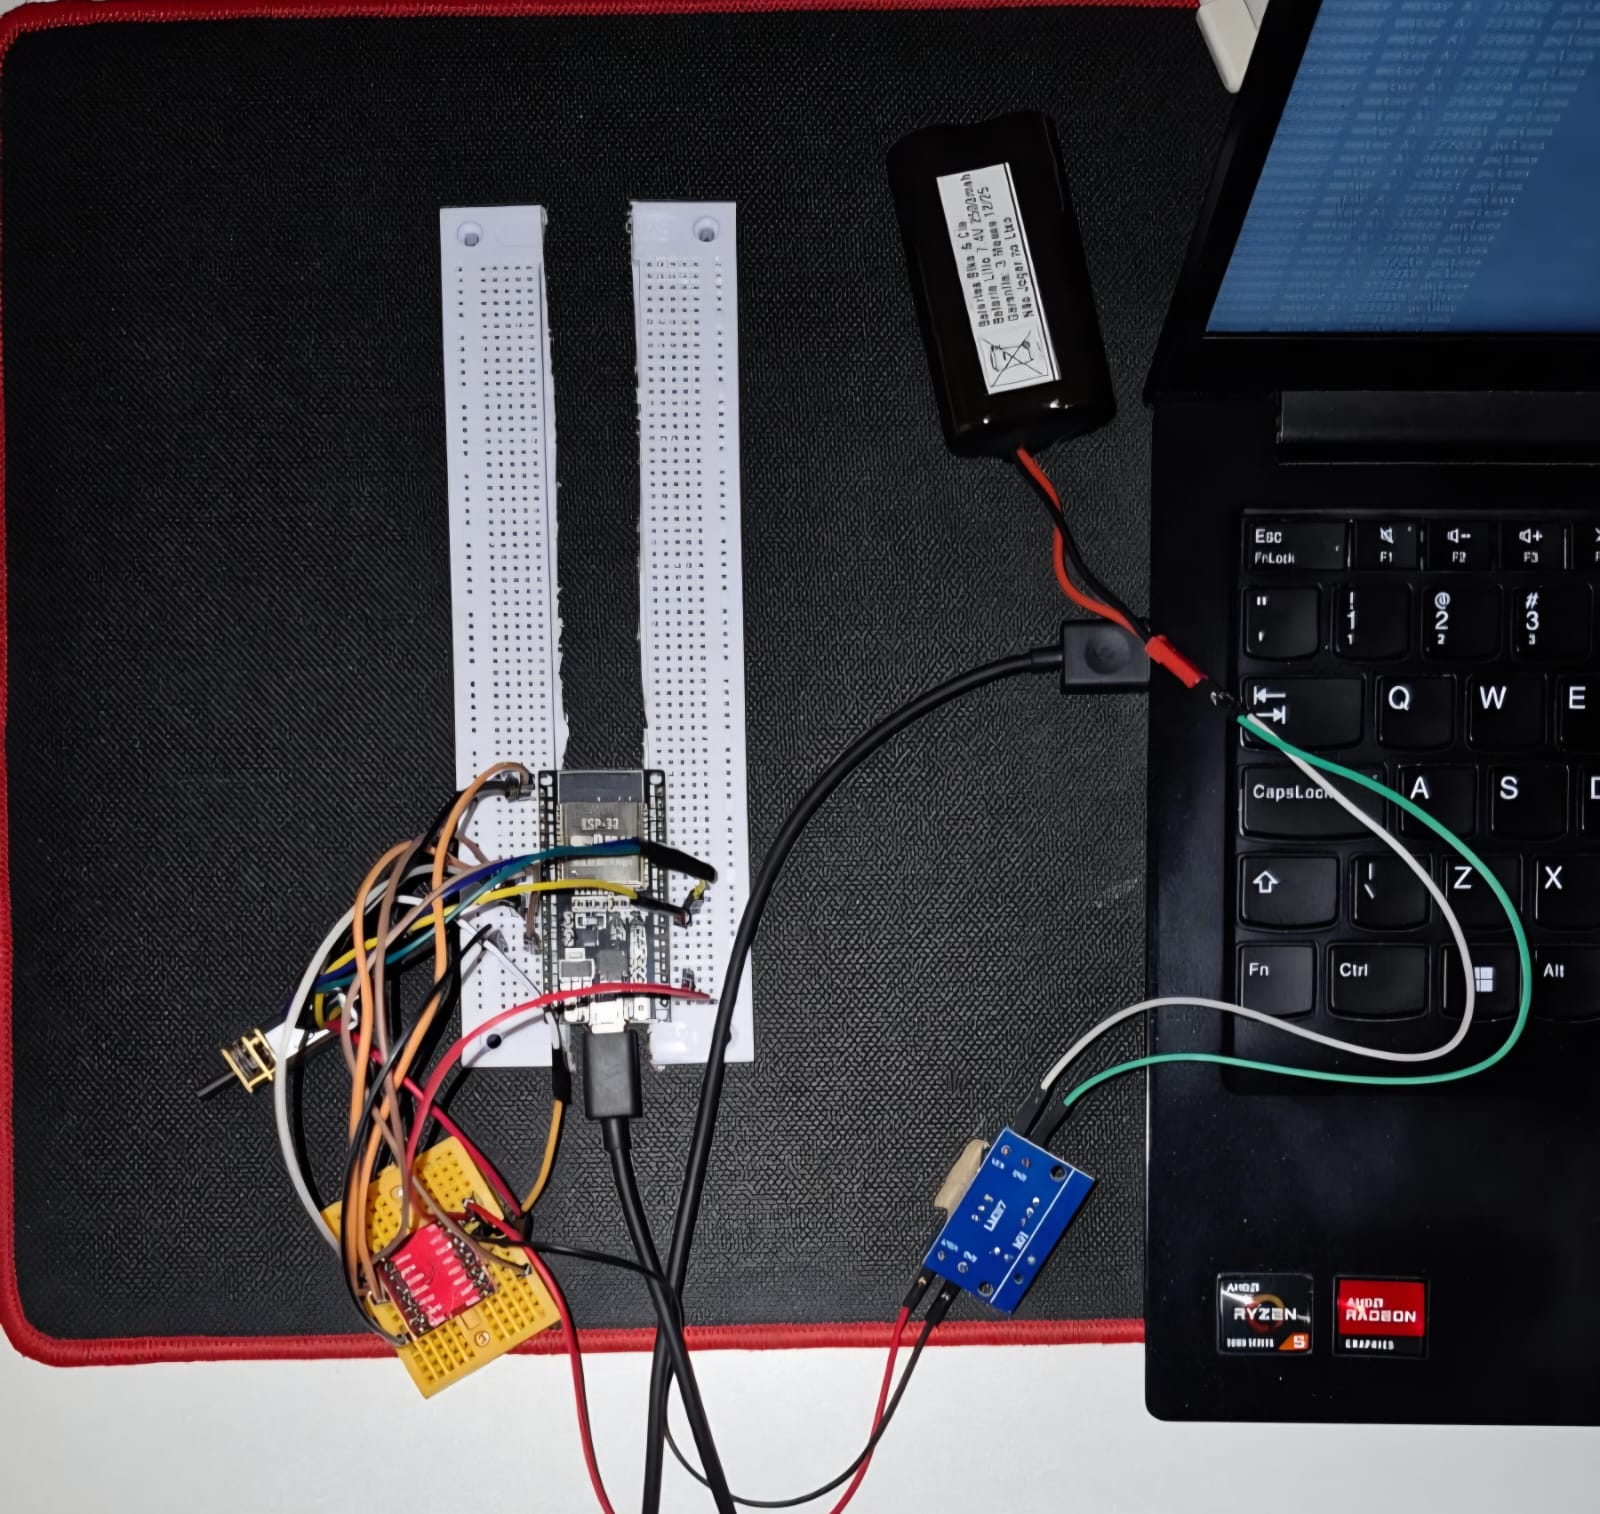
\includegraphics[width=0.8\textwidth]{figuras/exemplo-minimo-eletronica.jpeg}
    \caption{Teste de processamento de exemplo mínimo}
    \label{fig:exemploMin}
\end{figure}

\subsection{Sensores}

Os sensores utilizados pela equipe são: 
\begin{itemize}
    \item 1 INA219;
    \item 2 Encoders relacionados aos motores;
    \item 3 ToF VL53L0X.
\end{itemize}

\subsubsection{Leitura básica de dados}
Iniciamos os testes dos sensores com a realização de leitura básica dos dados dos sensores ToF, INA219 e dos encoders. Dessa forma, nessa primeira etapa, não foi feita a validação e calibragem das leituras, sendo o foco apenas a leitura dos dados. 

As Figuras \ref{fig:leituraToF}, \ref{fig:leituraINA} e \ref{fig:leituraEncoders} mostram a leitura básica de todos os sensores utilizados. Cabe lembrar que para os sensores que se repetem, colocamos apenas uma foto da execução do teste no relatório, porém todos foram testados e aprovados.

\begin{figure}[htbp]
    \centering
    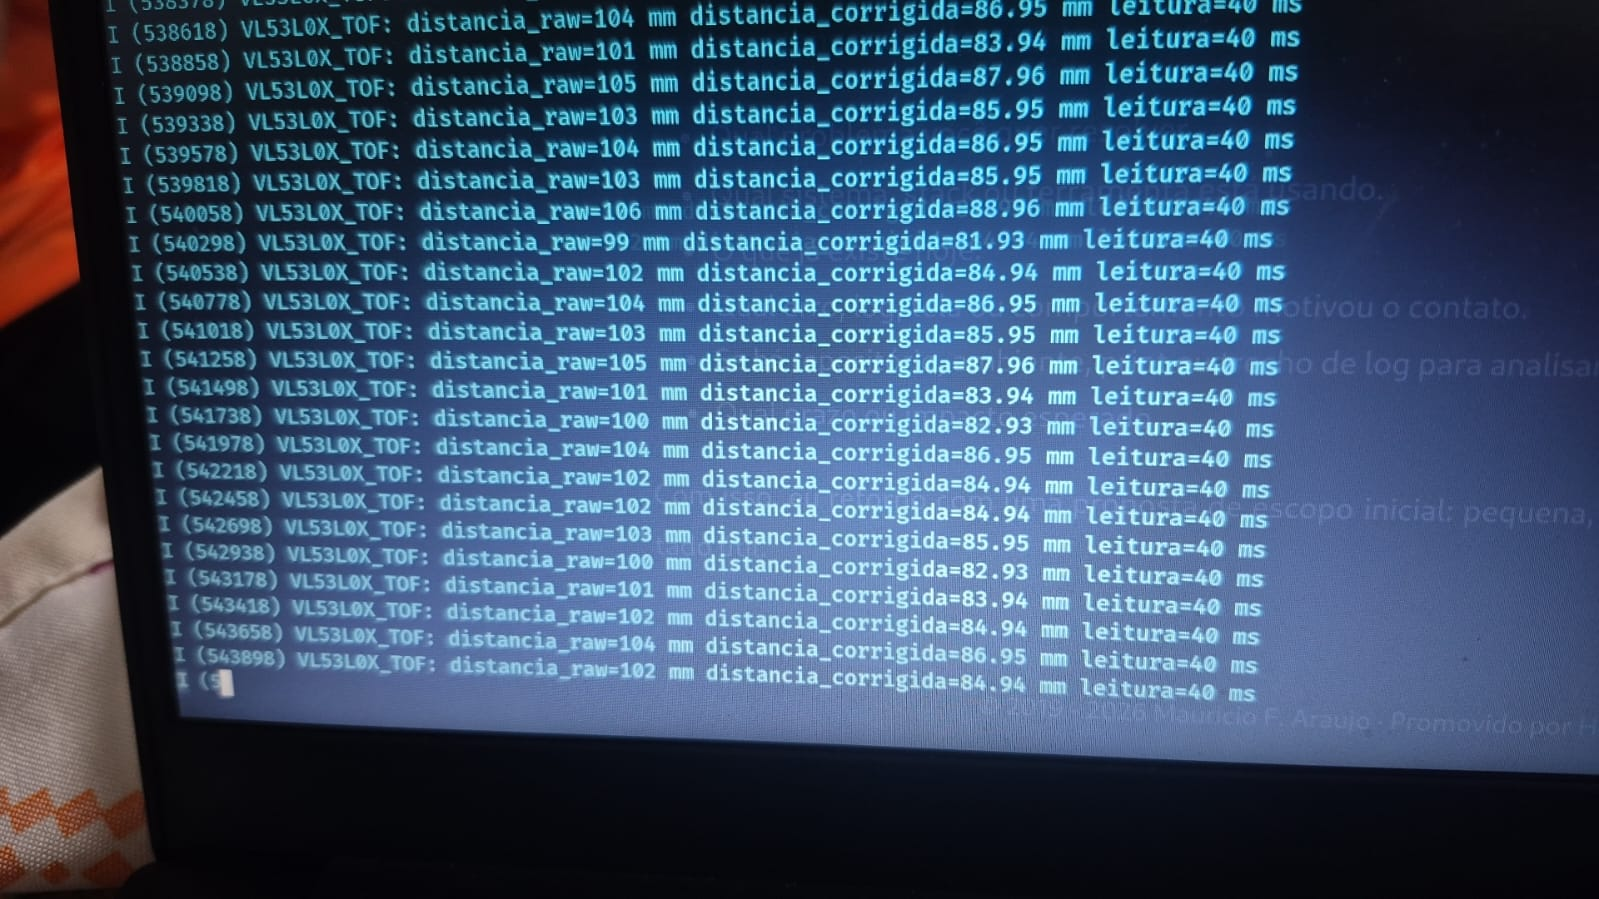
\includegraphics[width=0.8\textwidth]{figuras/TOFTeste.jpeg}
    \caption{Leitura básica do ToF}
    \label{fig:leituraToF}
\end{figure}

\begin{figure}[htbp]
    \centering
    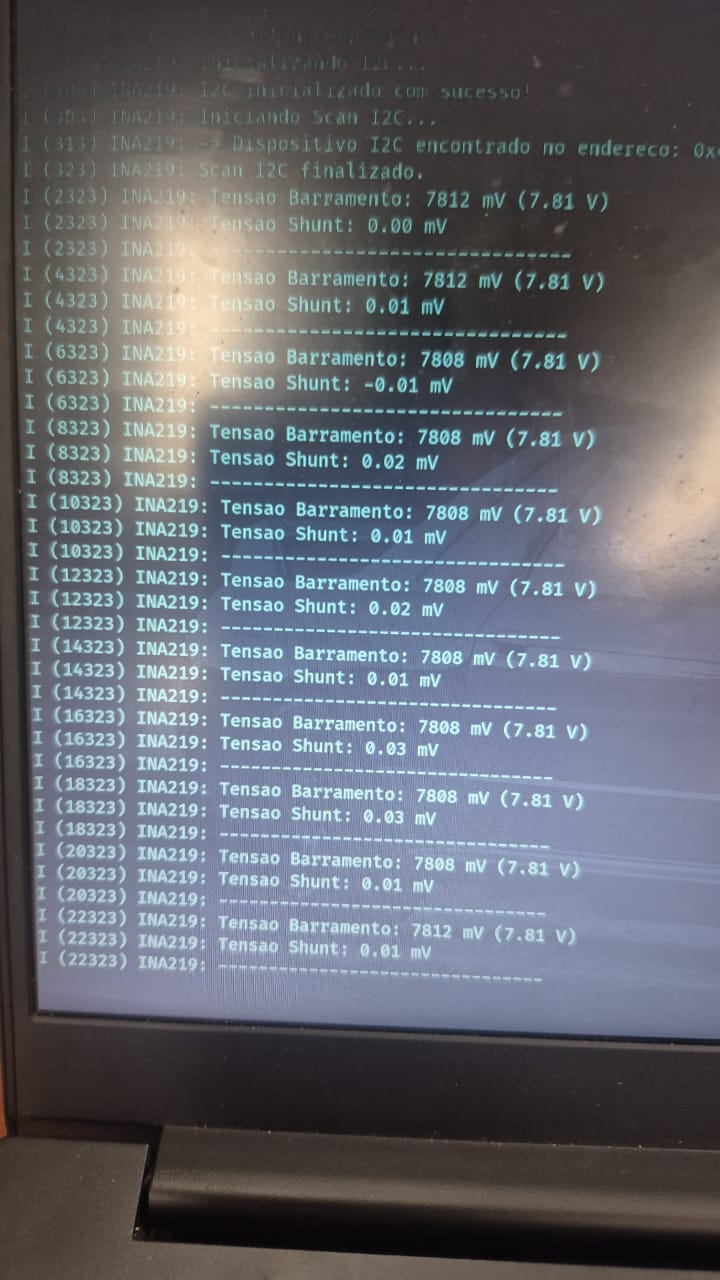
\includegraphics[width=0.8\textwidth]{figuras/INATeste.jpeg}
    \caption{Leitura básica do INA219}
    \label{fig:leituraINA}
\end{figure}

\begin{figure}[htbp]
    \centering
    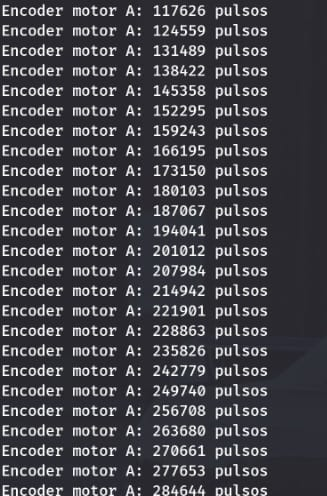
\includegraphics[width=0.8\textwidth]{figuras/encoderTeste.jpeg}
    \caption{Leitura básica dos encoders}
    \label{fig:leituraEncoders}
\end{figure}

\subsubsection{Validação e calibragem de leituras}

A calibragem dos sensores ToF foi feita a partir de medições reais comparadas com as medições do sensor, montamos primeiro um gráfico sendo o eixo x as medições reais, e o eixo y sendo as medições feitas pelo sensor ToF. Depois fizemos pelo método de regressão linear dos mínimos quadrados uma reta no formato $a \times x + b$ para achar a reta mais próxima. 

Por fim, chegamos a reta $0.9951 \times x + 17.475$, a qual usamos da seguinte forma para corrigir as leituras do sensor: $real = 0.9951 \times sensor - 17.475$; e depois aplicamos o filtro EMA \cite{pieterp_ema} que consistem em:

\begin{equation}
y[n] = \alpha x[n] + (1-\alpha)y[n-1]
\end{equation}

onde:
\begin{itemize}
    \item $y[n]$ medição filtrada, na iteração $n$;
    \item $x[n]$ valor real medido;
    \item $y[n-1]$ valor filtrado anteriormente;
    \item $\alpha$ fator de filtragem $0 \leq \alpha \leq 1$.
\end{itemize}

Para permitir que o robô realize curvas com ângulos específicos, irá adotada uma estratégia de calibração baseada na contagem de pulsos do encoder.

Como o sistema ainda não possui informações precisas sobre as dimensões mecânicas do conjunto de tração, optou-se por uma abordagem experimental. Inicialmente, os contadores de pulsos são zerados e o robô realiza uma rotação completa de 360° em torno do próprio eixo. Ao final da manobra, registra-se a quantidade total de pulsos gerados pelo encoder.

Esse valor passa a ser utilizado como referência para determinar a quantidade de pulsos necessária para qualquer outro ângulo de rotação. A relação é obtida por meio de uma regra de três:

$$
P_{\theta}=\frac{\theta \cdot P_{360}}{360}
$$

onde:
\begin{itemize}
    \item \(P_{360}\) é a quantidade de pulsos medida durante a rotação completa;
    \item \(P_{\theta}\) é a quantidade de pulsos correspondente ao ângulo desejado;
    \item \(\theta\) representa o ângulo de rotação solicitado.
\end{itemize}

A Figura \ref{fig:calibragemTOF} registra a calibragem feita para os sensores ToF. 

\begin{figure}[htbp]
    \centering
    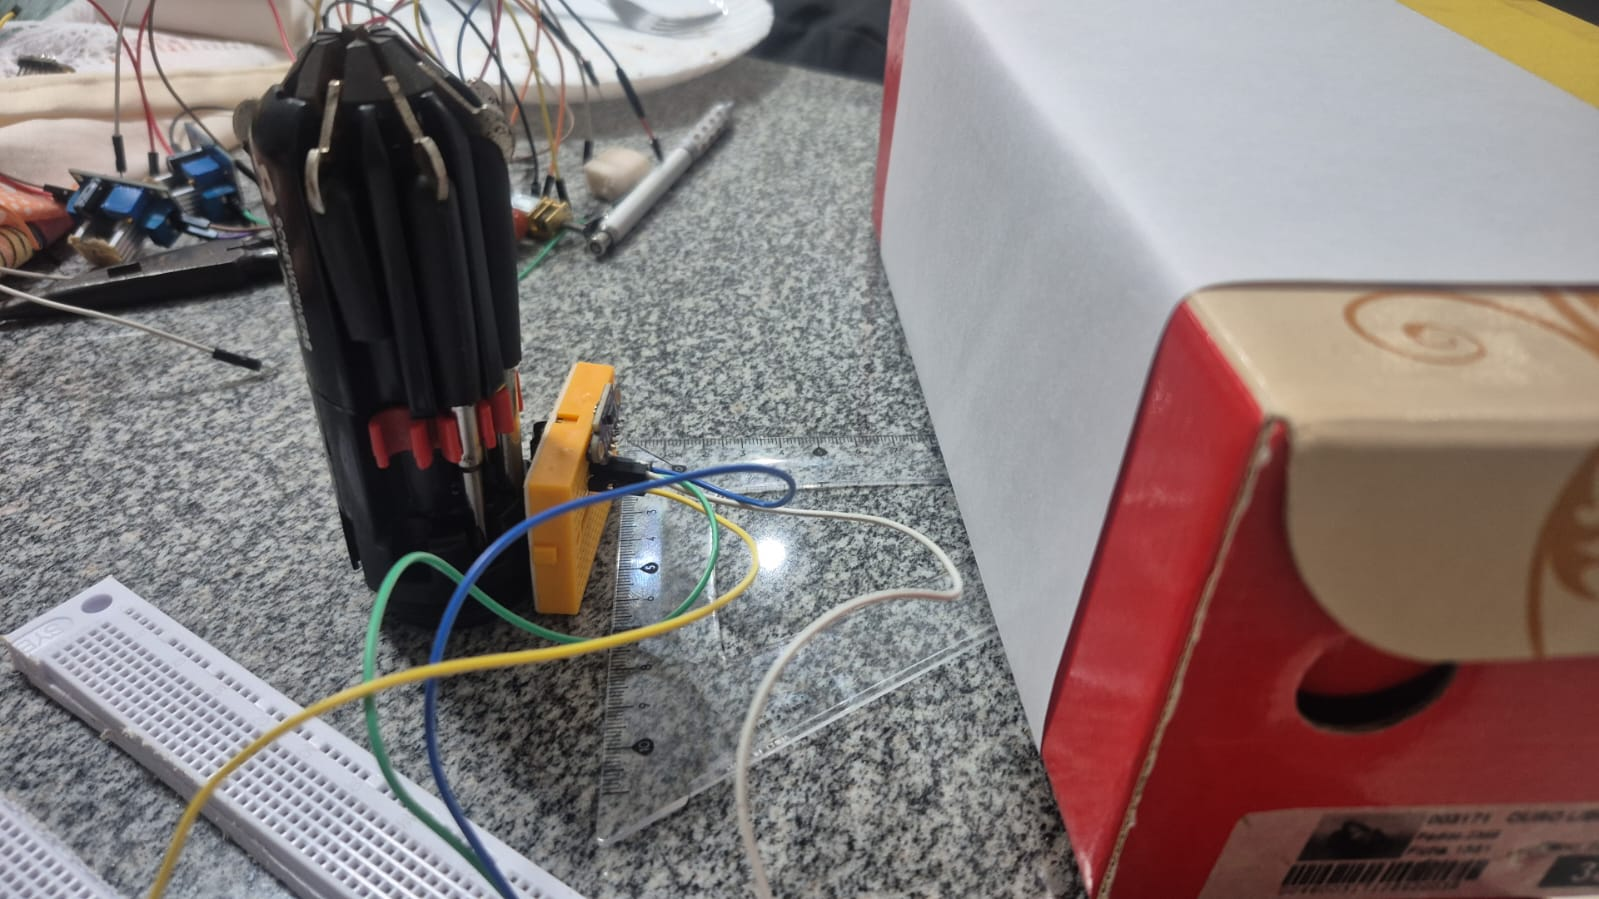
\includegraphics[width=0.8\textwidth]{figuras/calibragemTOF.jpeg}
    \caption{Realização da calibragem dos ToFs}
    \label{fig:calibragemTOF}
\end{figure}
    
\subsection{Armazenamento}

O armazenamento dos dados coletados pelos sensores está sendo feito a partir da telemetria com sockets UDP para o servidor web local na mesma rede WIFI que a ESP32 está conectada. Estamos utilizando oInfluxDB, um banco de dados de séries temporais, usado em projetos que armazenam dados que mudam em relação ao tempo, para persistência dos dados registrados pelos sensores utilizados para o funcionamento do MicroMouse.

\subsection{Comunicações}

A comunicação é feita via sockets UDP para o servidor \textit{backend} local em um computador conectado a mesma rede WIFI que a ESP32. Ela acontece em paralelo, pinada a um \textit{core} da ESP32 enquanto o processamento dos dados e tomadas de decisões acontece em outro \textit{core}.

\begin{comment}
\textcolor{red}{Apresentar com detalhes os testes feitos para conferir se os objetivos do \textit{hardware} foram atendidos, incluindo:}

\begin{enumerate}
    \item \textcolor{red}{Processamento (Arduino, ESP32 etc):}
    \begin{itemize}
        \item \textcolor{red}{Definir interface de desenvolvimento;}
        \item \textcolor{red}{Rodar exemplo mínimo.}
    \end{itemize}
    \item \textcolor{red}{Sensores (temperatura, pressão, posição, velocidade etc.):}
    \begin{itemize}
        \item \textcolor{red}{Realizar leitura básica de dados;}
        \item \textcolor{red}{Validar/calibrar leituras;}
        \item \textcolor{red}{Definir taxas de amostragem e quantidade de dados para transmissão e/ou armazenamento;}
        \item \textcolor{red}{Validar taxas definidas e quantidade de dados;}
        \item \textcolor{red}{Realizar processamento básico de dados (\textit{thresholding}, filtro média-móvel etc.).}
    \end{itemize}
    \item \textcolor{red}{Armazenamento (memória interna, cartão SD, pendrive etc.):}
    \begin{itemize}
        \item \textcolor{red}{Armazenar dados básicos;}
        \item \textcolor{red}{Armazenar e validar dados de sensores.}
    \end{itemize}
    \item \textcolor{red}{Atuadores (Motores DC, relés, LEDs etc.):}
    \begin{itemize}
        \item \textcolor{red}{Realizar acionamentos básicos;}
        \item \textcolor{red}{Realizar acionamentos com base em dados de sensores;}
        \item \textcolor{red}{Realizar processamento básico de dados (PWM etc.).}
    \end{itemize}
    \item \textcolor{red}{Comunicações (UART, I2C, SPI, USB, WiFi, Bluetooth etc.):}
    \begin{itemize}
        \item \textcolor{red}{Transmissão básica de dados;}
        \item \textcolor{red}{Transmissão de dados de sensores dentro da taxa de amostragem.}
    \end{itemize}
\end{enumerate}
\end{comment}

\section{Testes de consumo energético}

Os testes da área de energia têm como objetivo garantir que a bateria escolhida irá satisfazer os parâmetros levantados na fase de dimensionamento energético.

\subsection{Característica da bateria}

Primeiro foi conferido na embalagem do produto se certas características correspondiam com o que era esperado da bateria, as informações verificadas estão na tabela \ref{tab:caracteristicas_bateria_validadas}.

\begin{table}[htpb]
\begin{center}
\caption{Características da bateria escolhida.}
\label{tab:caracteristicas_bateria_validadas}
\begin{tabular}{|p{4cm}|p{4cm}|p{4cm}|}
\hline
\textbf{Parâmetro} & \textbf{Valor} & \textbf{Validado} \\ \hline
Química  & Lítio-Polímero (Lipo) & Sim \\ \hline
Configuração & 2 células & Sim\\ \hline
Tensão Nominal & $7,4V$ & Sim\\ \hline
Capacidade & $2200 mAh$ & Sim\\ \hline
\end{tabular}
\end{center}
\end{table}

\subsection{Teste em Repouso}

Depois da validação das especificações, foi feito o teste em repouso, afim de validar que a tensão da bateria era maior ou igual a tensão esperada. Foi utilizado um multímetro e a tensão medidda foi igual a $8,63 volts$, sendo validada a tensão em repouso uma vez que a tensão em repouso obtida é maior do que a esperada, que era de $7,4\ volts$. É possível visualizar o resultado na figura \ref{fig:Teste tensao bateria}.

    \begin{figure}[htbp]
        \centering
        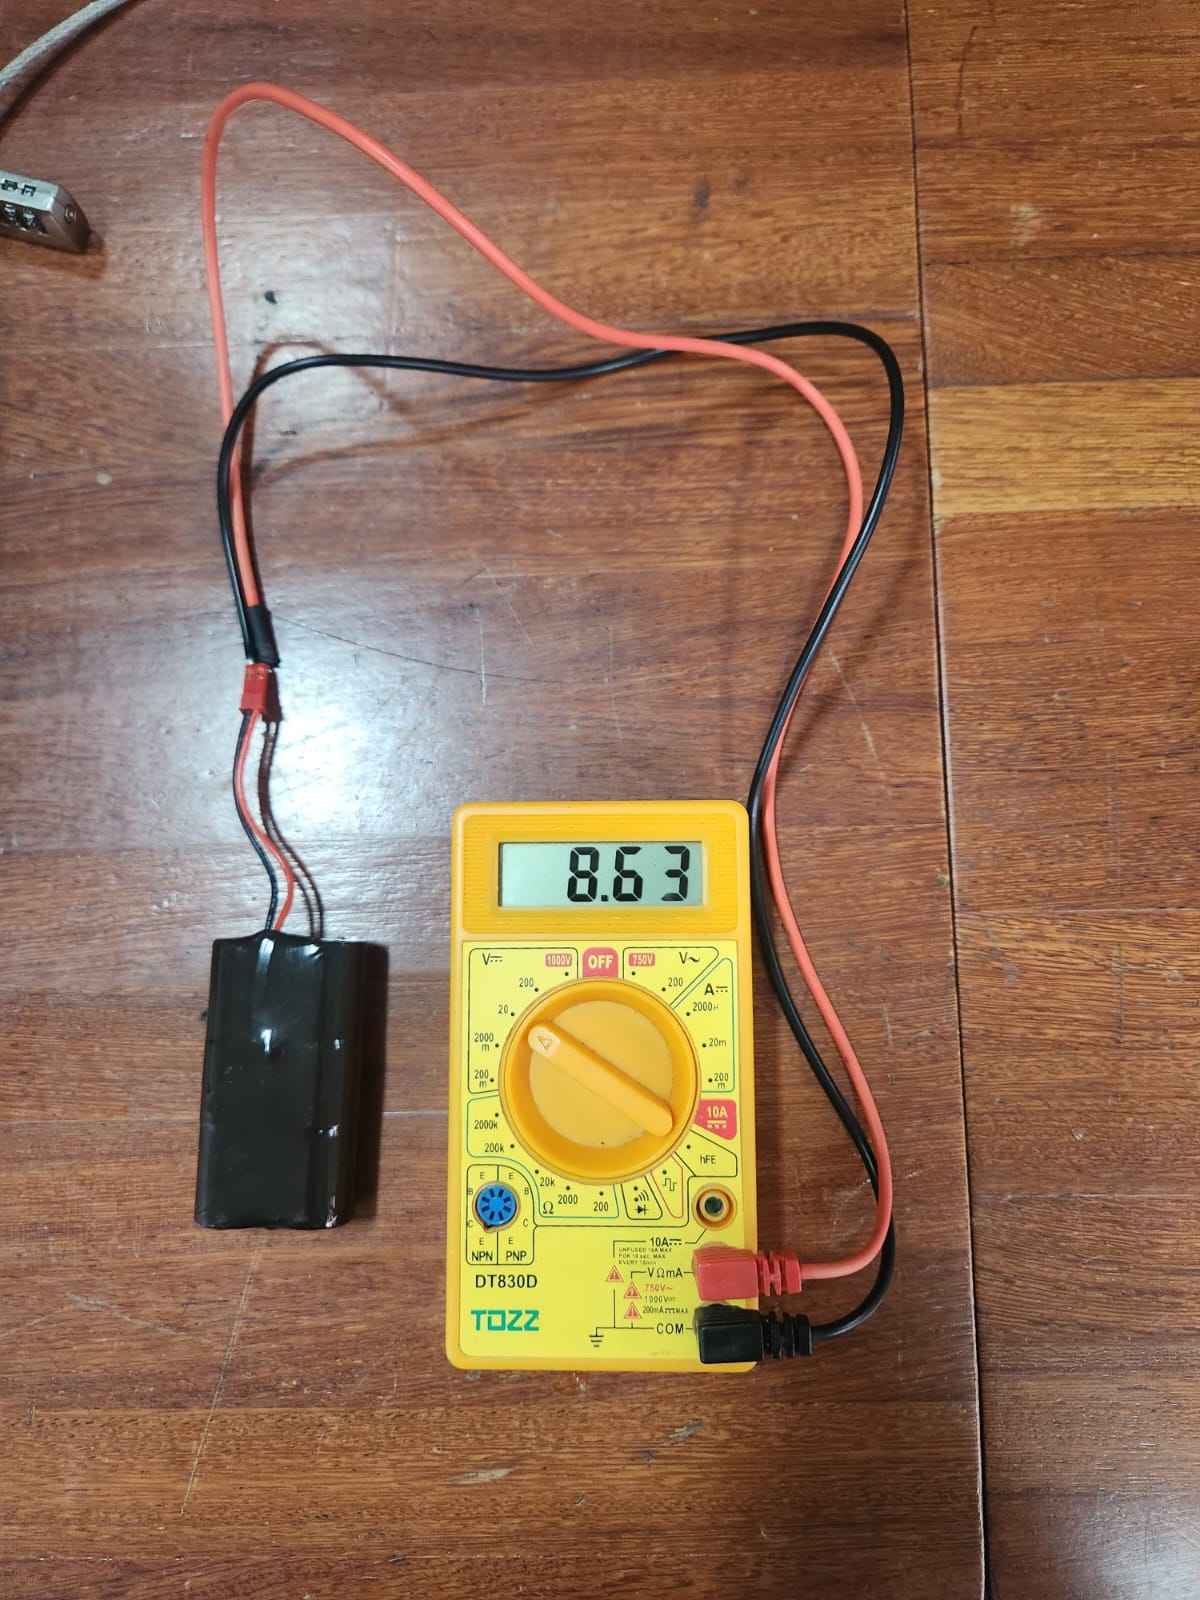
\includegraphics[width=0.25\textwidth]{figuras/teste_energia_tensao_bateria.jpeg}
        \caption{Tensão da bateria em repouso.}
        \label{fig:Teste tensao bateria}
    \end{figure}

\subsection{Teste de autonomia cronometrada}

Neste teste, o objetivo foi avaliar a capacidade de fornecimento de energia da bateria aos componentes eletrônicos do sistema. Durante a execução, algumas limitações estiveram presentes: o terceiro sensor ToF ainda não havia sido entregue e um dos motores não foi acionado no ensaio principal. Além disso, a ESP32 foi alimentada externamente via USB, de forma a manter o controle sobre a leitura e transmissão dos dados dos sensores ao computador sem interferir na medição de autonomia da bateria. Os componentes efetivamente alimentados por ela ao longo do experimento foram os dois sensores ToF, o módulo INA219 e um motor DC. Na Figura \ref{fig:Teste energia integrado} é possível visualizar o cronômetro e os componentes eletrônicos em operação durante o ensaio de 18 minutos.

Paralelamente, a bateria foi cedida à equipe de eletrônica para testes individuais e combinados realizados com uma única carga completa. Nesses ensaios adicionais, foram acionados componentes além dos presentes no teste principal, incluindo os dois motores operando simultaneamente. O conjunto de testes realizados, ainda que sem operar todos os componentes de forma integrada em um único ensaio, fornece respaldo suficiente para a equipe confiar que a bateria suportará a carga total do sistema ao longo de uma corrida completa.

    \begin{figure}[htbp]
        \centering
        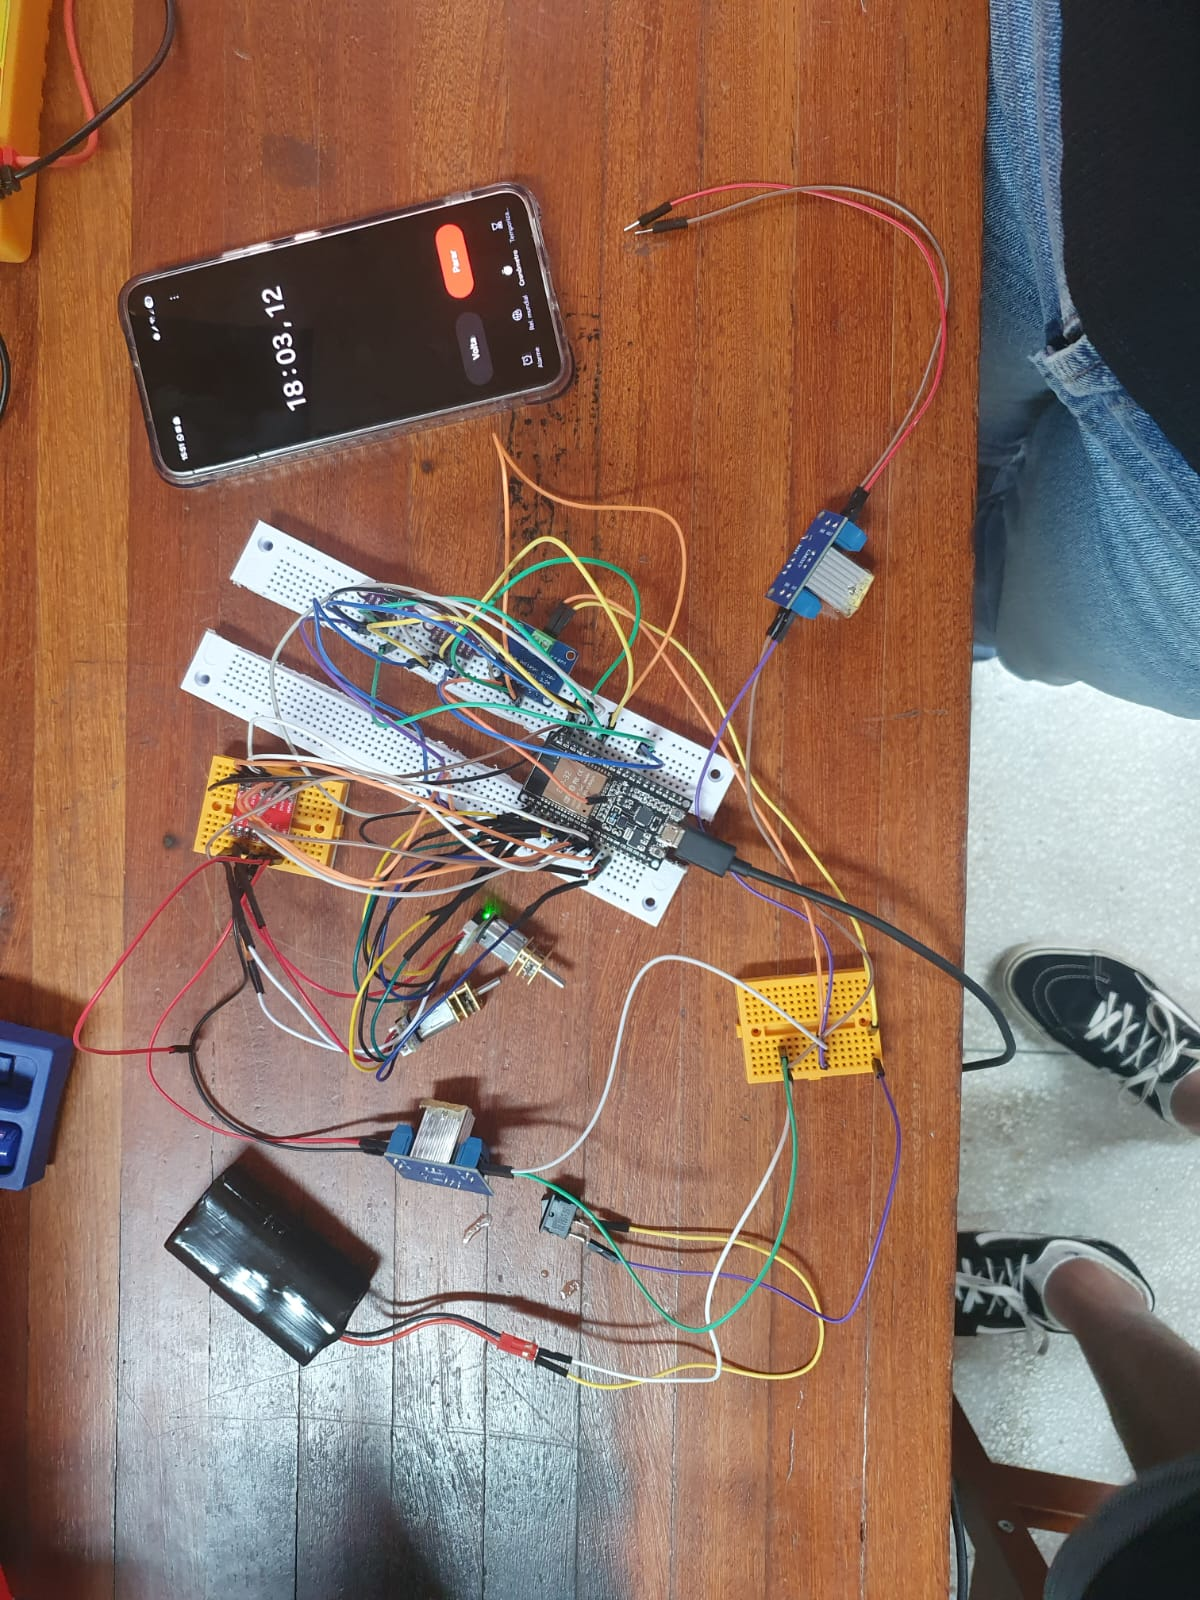
\includegraphics[width=0.3\textwidth]{figuras/teste_energia_integracao.jpeg}
        \caption{Sistema integrado}
        \label{fig:Teste energia integrada}
    \end{figure}

\section{Testes de \textit{software}}

\subsection{Histórias de Usuário Implementadas}

Das várias histórias de usuário (HUs) mapeadas no \textit{backlog} do projeto no GitHub, boa parte de sua fundação estrutural já foi implementada e exaustivamente testada nesta fase. A Tabela \ref{tab:historias_usuario_implementadas} lista as HUs principais deste pacote e como elas se materializam no sistema.

\begin{figure}[H]
    \centering
    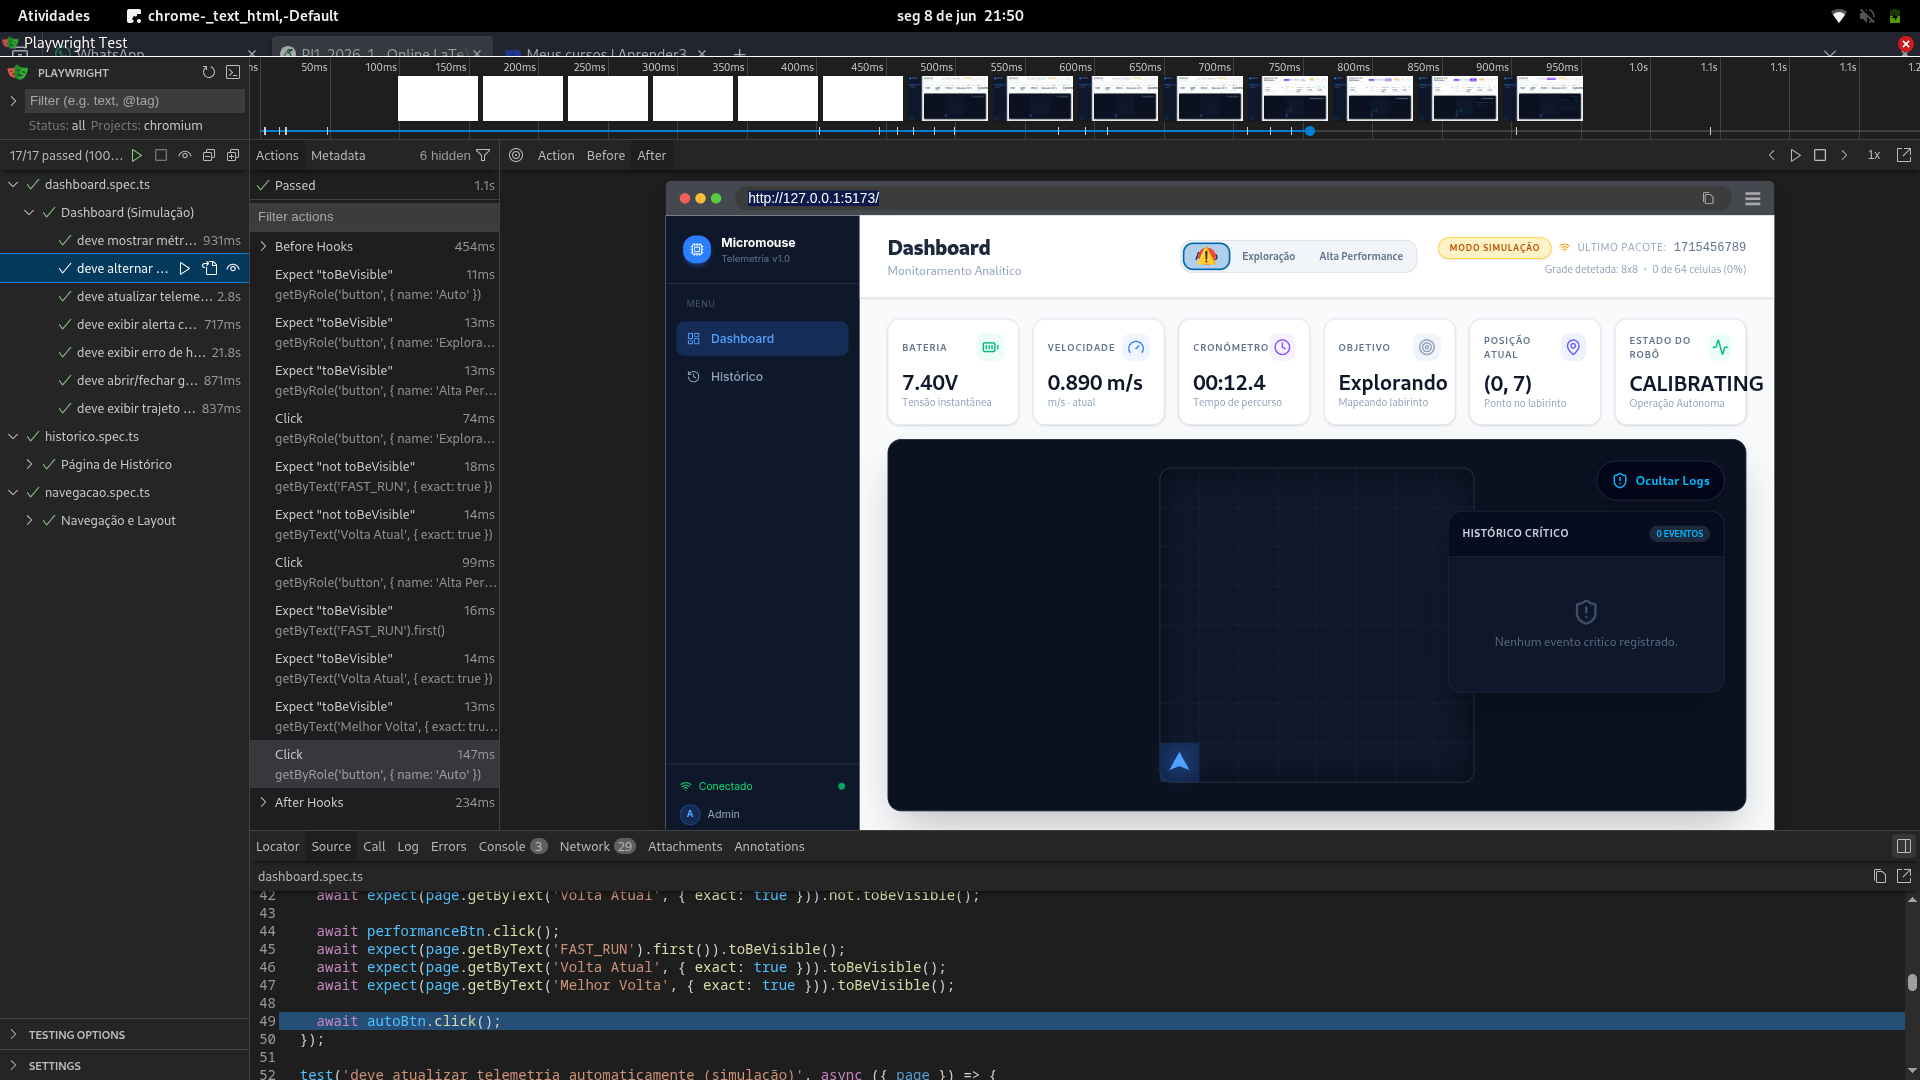
\includegraphics[width=0.5\linewidth]{figuras/teste_e2e_playwright.png}
    \caption{Execução de fluxos E2E no sistema.}
    \label{fig:placeholder}
\end{figure}

\begin{table}[H]
    \centering
    \caption{Histórias de Usuário Implementadas e Validadas}
    \label{tab:historias_usuario_implementadas}
    \begin{tabular}{|p{1.5cm}|p{6.5cm}|p{6cm}|}
        \hline
        \textbf{ID} & \textbf{Título da História} & \textbf{Validação / Interface} \\ \hline
        \textbf{HU 2.1.2} & Consumir telemetria do backend para acompanhar posição real & Dashboard: painel principal com representação matricial do robô. \\ \hline
        \textbf{HU 2.4} & Layout Adaptativo para Modo Alta Performance & Dashboard: botões de \textit{override} (Auto, Exploração, Alta Performance). \\ \hline
        \textbf{HU 3.1b} & Monitoramento Dinâmico da FSM & Dashboard: \textit{badge} dinâmico exibindo IDLE, MAPPING, etc. \\ \hline
        \textbf{HU 3.2} & Monitoramento de Tensão da Bateria & Dashboard: indicador numérico no \textit{header} com alerta crítico caso $V < 6.8$. \\ \hline
        \textbf{HU 3.5} & Plotagem em Tempo Real do Erro Direcional (PID) & Dashboard: gráficos reativos no painel de desempenho. \\ \hline
        \textbf{HU 3.6} & Alarme Imediato de Interrupção de Hardware & Dashboard: Modal \textit{pop-up} vermelho de ``Alarme Crítico''. \\ \hline
        \textbf{HU 4.1} & Gravação Contínua no InfluxDB & \textit{Backend}: fluxo UDP contínuo garantindo persistência. \\ \hline
        \textbf{HU 4.3} & Exportação de Histórico para Análise Externa & Página de Histórico: botão de \textit{Download CSV/JSON}. \\ \hline
        \textbf{HU 4.4} & Filtragem e Comparação de Desempenho por Pista & Dashboard: métricas de ``Volta Atual'' e ``Melhor Volta''. \\ \hline
        \textbf{HU 5.1.2} & Manter interface responsiva sem travamentos na queda de pacotes UDP & \textit{Frontend}: tratamento de jitter e tolerância a falhas na UI. \\ \hline
        \textbf{HU 6.1.2} & Validar propagação de pesos no simulador (Flood Fill) & \textit{Firmware}: Testes unitários com a biblioteca \textit{Catch2}. \\ \hline
    \end{tabular}
\end{table}

\subsection{Testes Unitários e Lógicos}

A equipe focou também em certificar a base lógica do robô, de forma isolada e em \textit{software}, para evitar problemas difíceis de depurar em hardware.

\subsubsection{Testes de Decodificação e Mapeamento (Backend)}
O módulo responsável por receber dados binários compactados no formato \textit{MessagePack} possui testes isolados no \textit{Jest}.
Foram validados pacotes corrompidos, decodificação correta de inteiros e valores em ponto flutuante, e tratativas de exceção (fallbacks de tempo) quando o robô envia métricas com chaves ausentes.

\begin{figure}[H]
    \centering
    % Cole a imagem do resultado do teste MsgPack com o nome abaixo:
    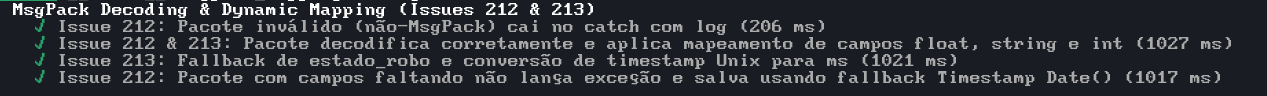
\includegraphics[width=0.8\textwidth]{figuras/teste_msgpack.png}
    \caption{Resultado da execução dos testes unitários de decodificação e mapeamento dinâmico (MsgPack) no Node.js.}
    \label{fig:teste_msgpack}
\end{figure}

\subsubsection{Testes de Front-end}

Os testes unitários do Front-end foram implementados com \textbf{Vitest} e \textbf{Testing Library}, cobrindo componentes React e funções utilitárias de forma isolada, sem dependência de rede ou estado externo. O ambiente de execução utiliza \textit{jsdom} para simular o DOM do navegador em Node.js. O resultado geral dessa suíte pode ser observado na Figura~\ref{fig:teste-cobertura-front-geral}.

\begin{figure}[H]
    \centering
    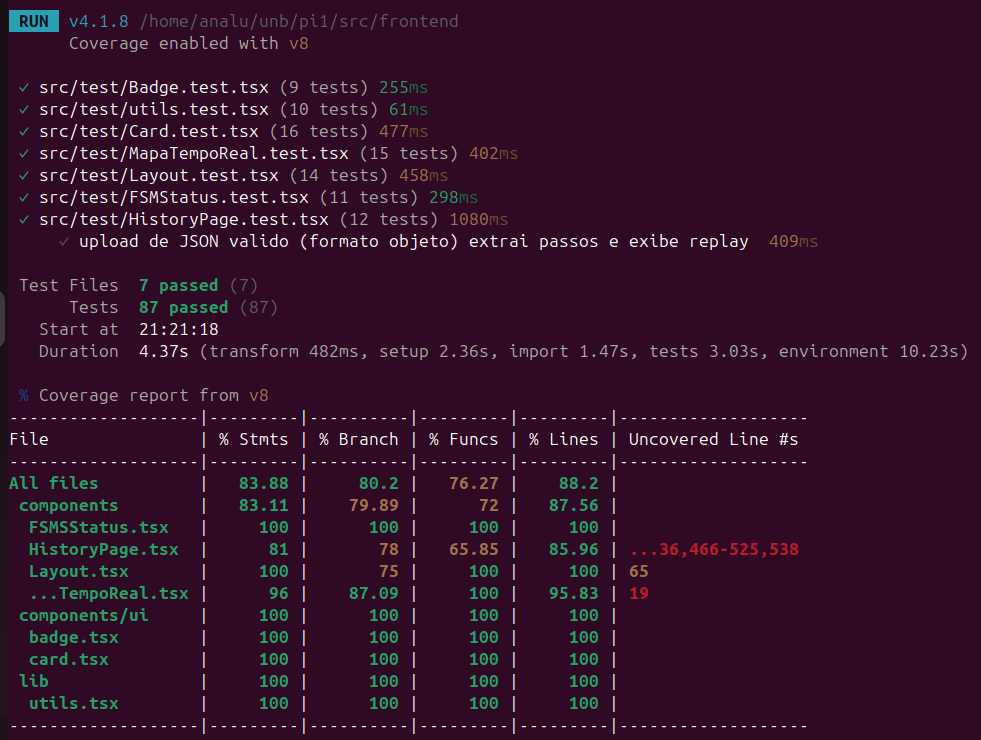
\includegraphics[width=0.7\textwidth]{figuras/cobertura-teste-frontend.png}
    \caption{Resultado geral dos testes unitários do Front-end.}
    \label{fig:teste-cobertura-front-geral}
\end{figure}

Com o objetivo de aumentar a testabilidade e garantir a pureza das funções, a lógica de manipulação da malha do labirinto foi recentemente refatorada. As funções foram extraídas do componente \texttt{HistoryPage.tsx} para o módulo utilitário independente \texttt{historyUtils.ts}. Foram implementados e validados 13 casos de teste focados nas operações primordiais desse módulo:

\begin{itemize}
    \item \textbf{Criação e Dimensionamento de Grid:} Geração de malhas bidimensionais vazias (\texttt{criarGridVazio}) com marcação precisa de bordas (para 4x4 e 16x16), além do arredondamento dinâmico das proporções do labirinto (\texttt{detectarTamanho}) para os padrões estruturais de 4, 8, 16 ou 32 células.
    \item \textbf{Manipulação Dinâmica do Labirinto:} Validação do espelhamento de obstáculos para as células vizinhas (\texttt{aplicarParede}) e reconstrução histórica do trajeto (\texttt{reconstruirAteStep}), atestando que todas as células visitadas são demarcadas corretamente até o passo analisado.
    \item \textbf{Parseamento e Formatação:} Extração segura do histórico de movimentos (\texttt{extrairPassos}) com tratamento adequado de exceções para formatos inválidos, e validação rigorosa via expressões regulares (\textit{Regex}) na formatação de \textit{timestamps} para atestar o padrão de datas pt-BR (\texttt{formatarTimestamp}).
\end{itemize}

É possível observar o resultado dessa suíte de testes recém-integrada e a respectiva cobertura de código na Figura~\ref{fig:teste-cobertura-history-utils}.

\begin{figure}[H]
    \centering
    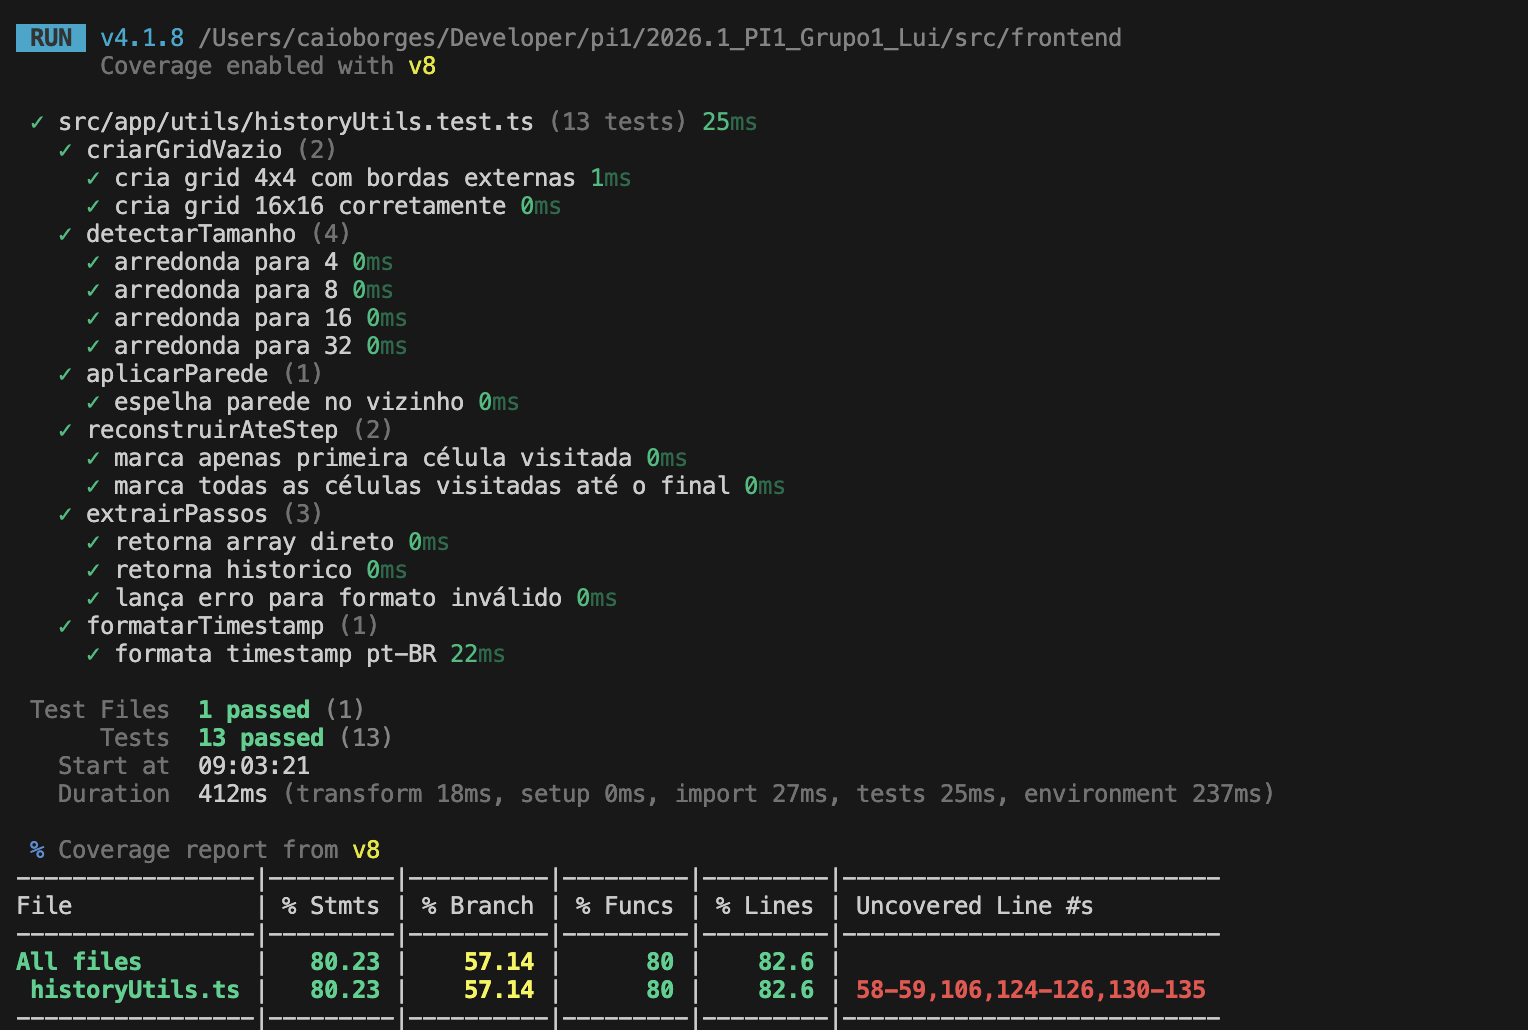
\includegraphics[width=0.7\textwidth]{figuras/cobertura-history-utils.png}
    \caption{Resultado e cobertura dos testes unitários do módulo \texttt{historyUtils}.}
    \label{fig:teste-cobertura-history-utils}
\end{figure}

\subsubsection{Testes Algorítmicos do Firmware (C++)}

O algoritmo principal de exploração (\textit{Flood Fill}), embarcado na ESP32, é isolado do hardware físico. Para atestar sua confiabilidade nas decisões de rotação e navegação, foi utilizada a biblioteca \textbf{Catch2}. 

O teste garante a corretude do recálculo da matriz de distâncias ao encontrar paredes e a lógica de prioridade de desempate (Frente $>$ Direita $>$ Esquerda $>$ Trás). É possível observar a execução bem-sucedida dos testes e que a cobertura de código atingiu $97\%$, conforme apresentado na Figura~\ref{fig:teste-cobertura-flood-fill}.

\begin{figure}[H]
    \centering
    % Cole a imagem do resultado do teste Catch2 com o nome abaixo:
    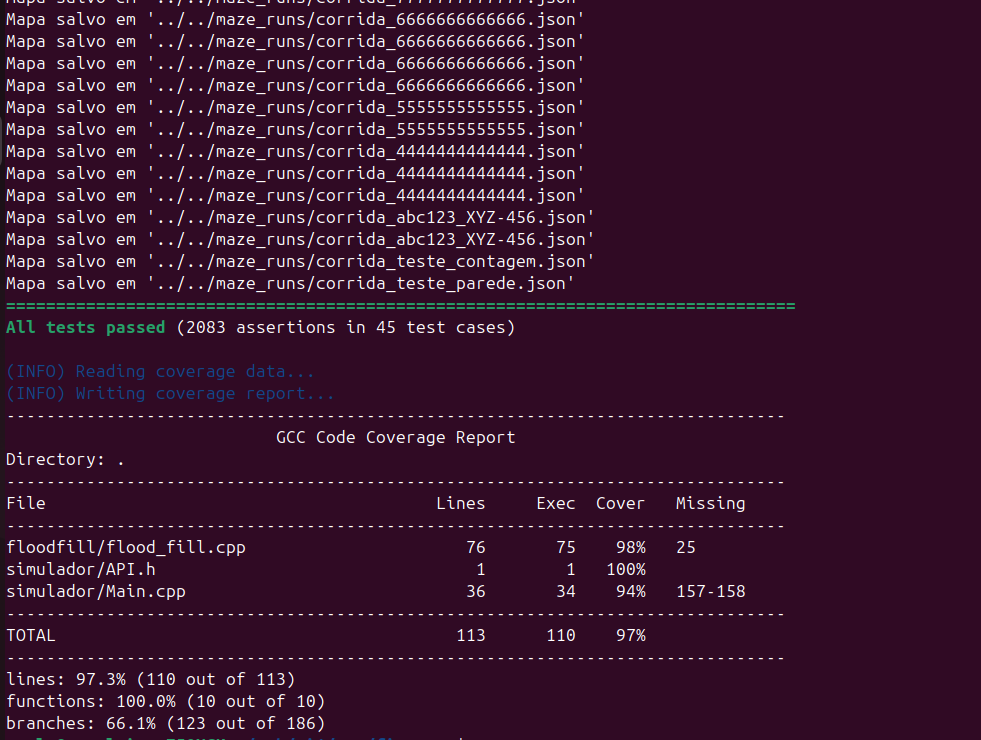
\includegraphics[width=0.7\textwidth]{figuras/cobertura-floodfill.png}
    \caption{Resultado dos testes unitários do algoritmo Flood Fill compilado e validado via \textit{framework} Catch2 e sua cobertura.}
    \label{fig:teste-cobertura-flood-fill}
\end{figure}

\subsection{Testes de Integração}

Dada a arquitetura fortemente acoplada a fluxos de dados em tempo real, foram desenhados \textbf{Testes de Integração} garantindo a resiliência do \textit{backend}. A ferramenta escolhida foi o \textbf{Jest}. Os testes automatizados garantem que pacotes UDP malformados não derrubem o servidor e que os dados válidos sejam persistidos corretamente no banco de dados temporal (\textit{InfluxDB}).

\begin{table}[H]
    \centering
    \caption{Casos de Teste de Integração (\textit{Backend})}
    \begin{tabular}{|p{3.5cm}|p{11.5cm}|}
        \hline
        \textbf{Integração Testada} & Módulo Servidor UDP (Node.js) $\leftrightarrow$ Banco de Dados (InfluxDB) \\ \hline
        \textbf{Ferramenta} & Jest (\texttt{integration.test.js}) \\ \hline
        \textbf{Cenário (Exemplo 1)} & \textbf{Rajada de Pacotes (Stress Test):} Envio sequencial de 10 pacotes de alta frequência simulando o modo FAST\_RUN. \\ \hline
        \textbf{Resultado Esperado} & O servidor deve \textit{flushar} os dados de forma assíncrona sem descartar pacotes (\textit{Zero Packet Loss}). \\ \hline
        \textbf{Cenário (Exemplo 2)} & \textbf{Falha no InfluxDB (Resiliência):} Simulação de indisponibilidade do banco de dados ao tentar registrar telemetria. \\ \hline
        \textbf{Resultado Esperado} & O \textit{backend} deve capturar a exceção e emitir log de erro sem fechar o processo Node.js (\textit{crash prevention}). \\ \hline
        \textbf{Resultado Obtido} & \textbf{APROVADOS}. A cobertura deste fluxo atende $100\%$ das rotas críticas do servidor. \\ \hline
    \end{tabular}
\end{table}

\begin{figure}[H]
    \centering
    % Cole a imagem do resultado do teste de integração com o nome abaixo:
    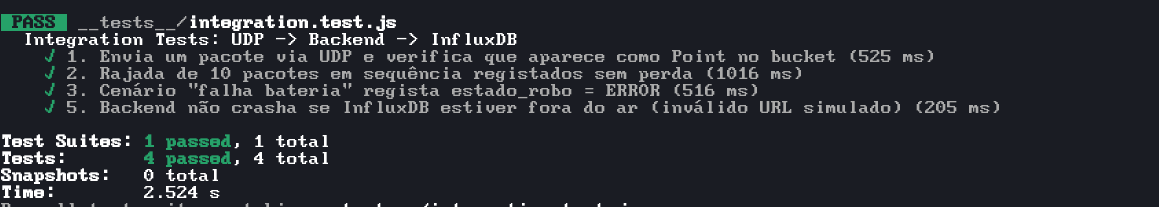
\includegraphics[width=0.8\textwidth]{figuras/teste_integracao_udp.png}
    \caption{Resultado da execução dos testes de integração garantindo o duto UDP e banco de dados InfluxDB.}
    \label{fig:teste_integracao}
\end{figure}

\subsection{Testes de Sistema (End-to-End)}

Para garantir a confiabilidade da interface gráfica sob a ótica do usuário, foram desenvolvidos testes funcionais automatizados (\textit{End-to-End}) utilizando o \textbf{Playwright}. Os testes replicam fluxos de interação reais no navegador web.

\begin{table}[H]
    \centering
    \caption{Casos de Teste E2E Funcional (\textit{Frontend})}
    \begin{tabular}{|p{3.5cm}|p{11.5cm}|}
        \hline
        \textbf{Fluxos Testados} & \textit{Dashboard} de Telemetria, Alertas Críticos, Navegação e Histórico. \\ \hline
        \textbf{Ferramenta} & Playwright (\texttt{dashboard.spec.ts}, etc.) \\ \hline
        \textbf{Cenário (Exemplo 1)} & \textbf{Renderização de Alerta de Hardware:} O sistema recebe um pacote cujo estado da FSM seja \texttt{ERROR}. \\ \hline
        \textbf{Resultado Esperado} & A tela deve exibir o modal de ``Alarme Crítico de Hardware'' com a causa base (ex: Parada de Emergência). \\ \hline
        \textbf{Cenário (Exemplo 2)} & \textbf{Troca de Modos de Operação:} O usuário clica no botão ``Alta Performance''. \\ \hline
        \textbf{Resultado Esperado} & A interface deve adaptar-se, ocultando métricas irrelevantes e destacando ``Volta Atual'' e ``Melhor Volta''. \\ \hline
        \textbf{Resultado Obtido} & \textbf{APROVADOS}. O sistema atendeu perfeitamente ao roteiro de testes visuais estabelecido. \\ \hline
    \end{tabular}
\end{table}

\begin{figure}[H]
    \centering
    % Cole a imagem do resultado do teste do Playwright com o nome abaixo:
    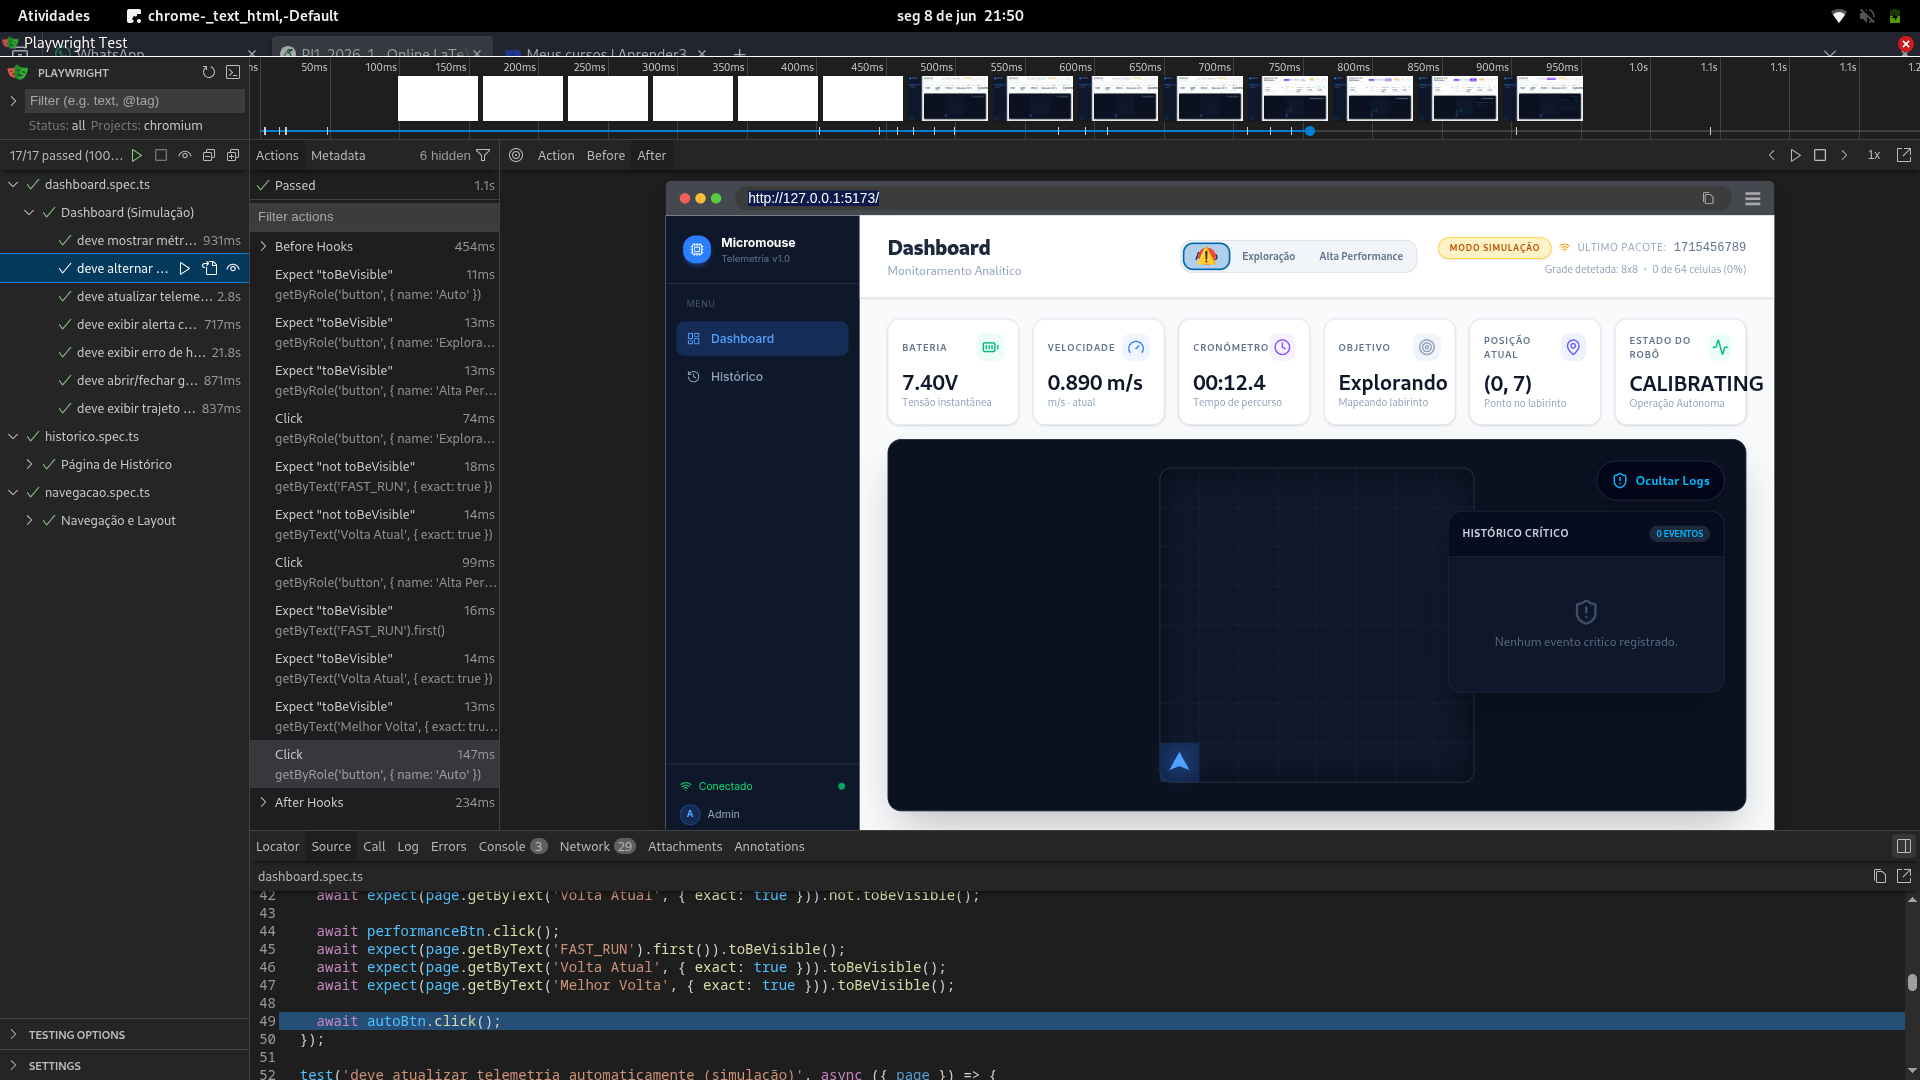
\includegraphics[width=0.8\textwidth]{figuras/teste_e2e_playwright.png}
    \caption{Resultado da execução automatizada de fluxos do usuário via Playwright.}
    \label{fig:teste_e2e}
\end{figure}

\section{Testes de Integração Global (Hardware e Software)}

Nesta seção é detalhado o teste final de integração global, onde os subsistemas de Estrutura, Eletrônica e Software do Micromouse operam em uníssono. O objetivo deste teste foi atestar a capacidade da arquitetura do robô em ler estímulos físicos contínuos, processá-los embarcadamente e transmiti-los via rede para visualização remota interativa, validando o conceito do projeto.

\textbf{Procedimento do Teste Global:}
\begin{enumerate}
    \item O robô foi posicionado em bancada de testes/corredor e energizado pela bateria principal de 7.4V.
    \item A placa \textit{ESP32} realizou o \textit{boot}, efetuou a estabilização e leitura inicial dos sensores e conectou-se com sucesso à rede Wi-Fi local.
    \item Simultaneamente, o servidor receptor em \textit{Node.js} e a interface \textit{React} (Frontend) foram inicializados em um \textit{host} ouvindo na mesma rede local.
    \item O robô iniciou a transmissão contínua de pacotes UDP formatados contendo dados de odometria (encodes), medições dos três sensores \textit{Time of Flight} (ToF), além dos estados dinâmicos da FSM e os níveis da bateria Li-ion.
\end{enumerate}

\textbf{Resultados Alcançados:}
Logo após a conexão, o painel \textit{Dashboard} da aplicação web exibiu de imediato o indicador de tensão medido (com nível superior a $7.4V$) e começou a desenhar a posição virtual do Micromouse em um \textit{canvas} interativo. Conforme o robô transitava fisicamente por modos distintos (de \texttt{IDLE} para \texttt{MAPPING} ou \texttt{FAST\_RUN}), a mudança era refletida instantaneamente na visualização \textit{web}. 

Não ocorreu descarte substancial de \textit{datagramas} UDP, nem foram detectados gargalos sistêmicos (excesso de requisições travando o DOM do React) ou \textit{delays} desproporcionais de \textit{parsing} no InfluxDB. A integração validou a viabilidade completa do conceito do robô, confirmando que o duto de processamento paralelo estabelecido em toda a linha de dados (\textit{Sensores} $\rightarrow$ \textit{ESP32 (C++)} $\rightarrow$ \textit{Comunicação UDP (WiFi)} $\rightarrow$ \textit{Backend (Node.js)} $\rightarrow$ \textit{Séries Temporais (InfluxDB) e Frontend (React)}) opera de forma coesa, com baixíssima latência e atende todos os requisitos arquiteturais previstos para o projeto.